\subsection{Empfangen der Messwerte}

\subsubsection{BLE Clients mit Python}
tbd: Ursprünglich: Python, Probleme mit Libaries, was wäre Vorteil gewesen wenn es funktioniert hätte...)
%TODO

\subsubsection{Alternativ Client zum Empfang der Daten per BLE: Android App}
\label{AndroidAppFürDatenmessen}
Da es bereits die Android-App ,,Adafruit Bluefruit LE Connect'' gibt, mit der Daten per BLE empfangen und gesendet werden können, konnte davon ausgegangen werden, dass in der Konstellation Smartphone-Bluefruit-Modul BLE-Verbindungen funktionieren und unterstützt werden. Daraus ergibt sich auch der Vorteil, dass ein Smartphone als Empfänger wesentlich mobiler ist, um an der Anlage am Sender mitlaufen zu können. 

Von Adafruit gibt es über Github\footnote{Github-Link: \url{https://github.com/adafruit/Adafruit_Android_BLE_UART}} die Klasse ,,Adafruit Android BLE UART'', mit der eine BLE-Verbindung zu einem Bluefruit-Modul von einem Android-Smartphone aus hergestellt werden kann. Dabei handelt es sich um eine abgespeckte Variante der App oben erwähnten App. Mit Hilfe des Codes für BLE-UART-Verbindungen wurde eine App entwickelt. Als Entwicklungsumgebung kam Android Studio zum Einsatz. Neben dem BLE-Aufbau muss die App Befehle an den Mikrocontroller senden können. Sobald Sensordaten vom Mikrocontroller ankommen, sollen diese Werte in lokalen Dateien gespeichert werden.

Zuerst musste eine Verbindung mit dem Bluefruit-Modul hergestellt werden. Bei eingeschaltetem Bluetooth am Smartphone sucht die App automatisch nach BLE-Geräten. 

Die App verfügt über vier Buttons, um das Verhalten des Mikrocontrollers sowie das Speichern der Daten kontrollieren zu können:
\begin{description}
	\item[Start] Sendet einen Start-Befehl an den Mikrocontroller, damit dieser mit dem Senden von gemessenen Sensordaten beginnt
	\item[Stop] Sendet einen Stop-Befehl an den Mikrocontroller, damit dieser mit dem Senden von gemessenen Sensordaten stoppt. Die gemessenen Daten bleiben dabei in einem String Buffer vorhanden
	\item[Save] Speichert die gemessenen Daten in einem neuen File ab. Dabei werden genutzte Zähler nicht zurückgesetzt. Der Button kann benutzt werden, um bei einem Messlauf markante Punkte performant zu markieren, indem ein neues File erstellt wird.
	\item[Reset \& Save] Speichert die gemessenen Werte in ein File und setzt anschließen genutzte Zähler zurück. Zusätzlich wird ein Reset-Befehl an den Mikrocontroller gesendet, um die BLE-Verbindung neuzustarten und ebenfalls Zähler zurückzusetzen. Bei erfolgreicher Wiederverbindung, beginnt direkt wieder der Datenempfang, sofern der Mikrocontroller vorher auch im Senden-Modus war. Der Button kann benutzt werden, um bei einem Messlauf eine neue Runde auf der Anlage zu markieren, sowie eine gute Performanz zu behalten, indem gespeicherte Felder nicht zu groß werden.
\end{description}

\begin{figure}[h]
	\centering
	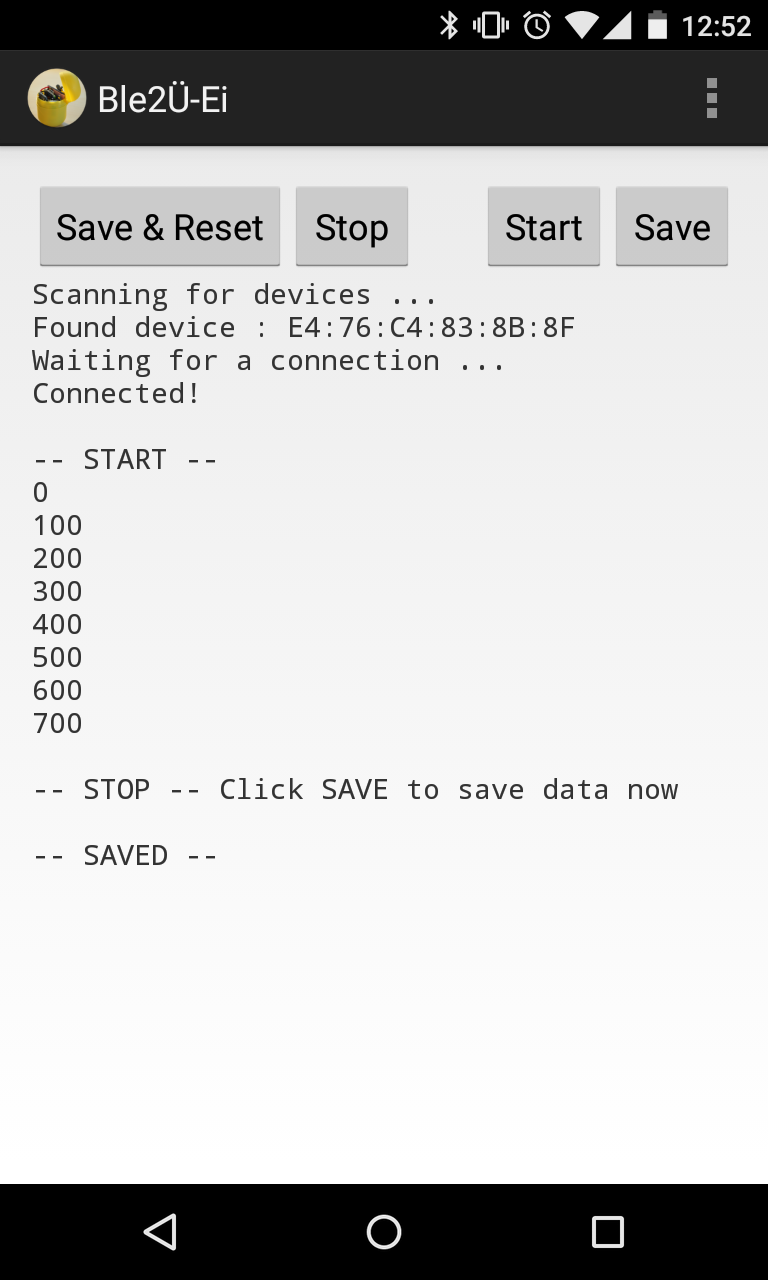
\includegraphics[width=0.5\textwidth]{images/k3-androidapp.png}
	\caption {Android-App zum Steuern des Mikrocontrollers und Empfangen der Sensordaten}
	\label{fig:k3_androidapp}
\end{figure}

Die Daten werden in Dateien lokal auf dem Smartphone gespeichert und müssen anschließend auf einen Rechner übertragen werden. Derzeit ist der ,,Download''-Ordner des Smartphones fest implementiert. Hier gibt es sicher noch Potential zur Erweiterung, indem die Daten direkt über einen Data Service an einen PC oder Laptop weitergeleitet werden könnten oder zumindest der Speicherort variabler wird. \\
Abgelegt werden die Files in einem bestimmten Namensformat. Sie beginnen mit dem aktuellen Timestamp um identische Filenamen zu verhinden. Zusätzlich wird noch der Bereich mittels eines internen App-Zählers angegeben, um zusammenhängende Dateien für eine Messrunde identifizieren zu können.